%==============================================================================
% Mini Preamble.
%==============================================================================

\documentclass[11pt]{article} % 10pt article, want AMS fonts.
\makeatletter					% Make '@' accessible.
\pagestyle{myheadings}				% We do our own page headers.
\skip\footins=4ex				% Space above first footnote.
\hbadness=10000					% No "underfull hbox" messages.
\makeatother					% Make '@' special again.
\usepackage{fullpage}
\usepackage{graphicx}
%==============================================================================
% Title.
%==============================================================================

\begin{document}
\centerline{\LARGE{CSCI 2951-F Final Project}}
\centerline{Enrique and Ellis and Kavosh and Dave}
\vspace{2mm}


% --- SECTION: Paper Overview ---
\section{Paper Overview}

Note: Introduce the problem that they're solving, i.e. identify the main research contribution made (a natural language version of theorem 1 ish? that there is this relationship between model accuracy and planning depth, and that gamma lets you control that).


% --- SECTION: Domains ---
\section{Domains}

% Section: Rock Sample
\subsection{RockSample}
The RockSample domain consists of an agent acting in a partially observable GridWorld bounded by walls on the west, south and north sides. There are $k$ rocks that occupy unique cells of the grid world some of which are good and some of which are bad. There are $5+k$ actions available to the agent, $\{North, East, South, West, Sample, Check_1 \ldots Check_k\}$. 

If the agent calls $Sample$ while it is on top of a good rock it receives $+10$ reward and if it does so while on top of a bad rock it receives $-10$ reward. The agent also receives $+10$ reward if it runs of the east edge of the GridWorld, thereby terminating the episode.

The state space is fully observable to the agent except the goodness of rocks -- that is, it always knows its own position and that of all rocks, but not the goodness of the rocks. The $Check_i$ action provides the agent with noisy knowledge of the $i$th rock. If the agent is directly on top of $rock_i$ the $Check$ action returns the true goodness of the rock. As the agent gets further and further from the rock that it is $Check$ing, the fidelity of its sensor falls off exponentially, bottoming out at a $50\%$ probability of returning the true goodness of the rock it is $Check$ing. The agent's initial belief state is that each rock has a $50\%$ chance of being good.

% Section: Randomized MDPs
\subsection{Randomized MDPs}



% --- SECTION: Hypotheses ---
\section{Hypotheses}

% Subsection: Figure 6
\subsection{Figure 6}

% Subsection: Figure 7
\subsection{Figure 7}


% --- SECTION: Experiments ---
\section{Experiments}

Idea: Discuss how we chose to implement our version of the experiments?



% --- SECTION: Results ---
\section{Results}

Summary of their results, summary of our results.

Cross validation with RandomMDP
$$\begin{tabular}{cc}
	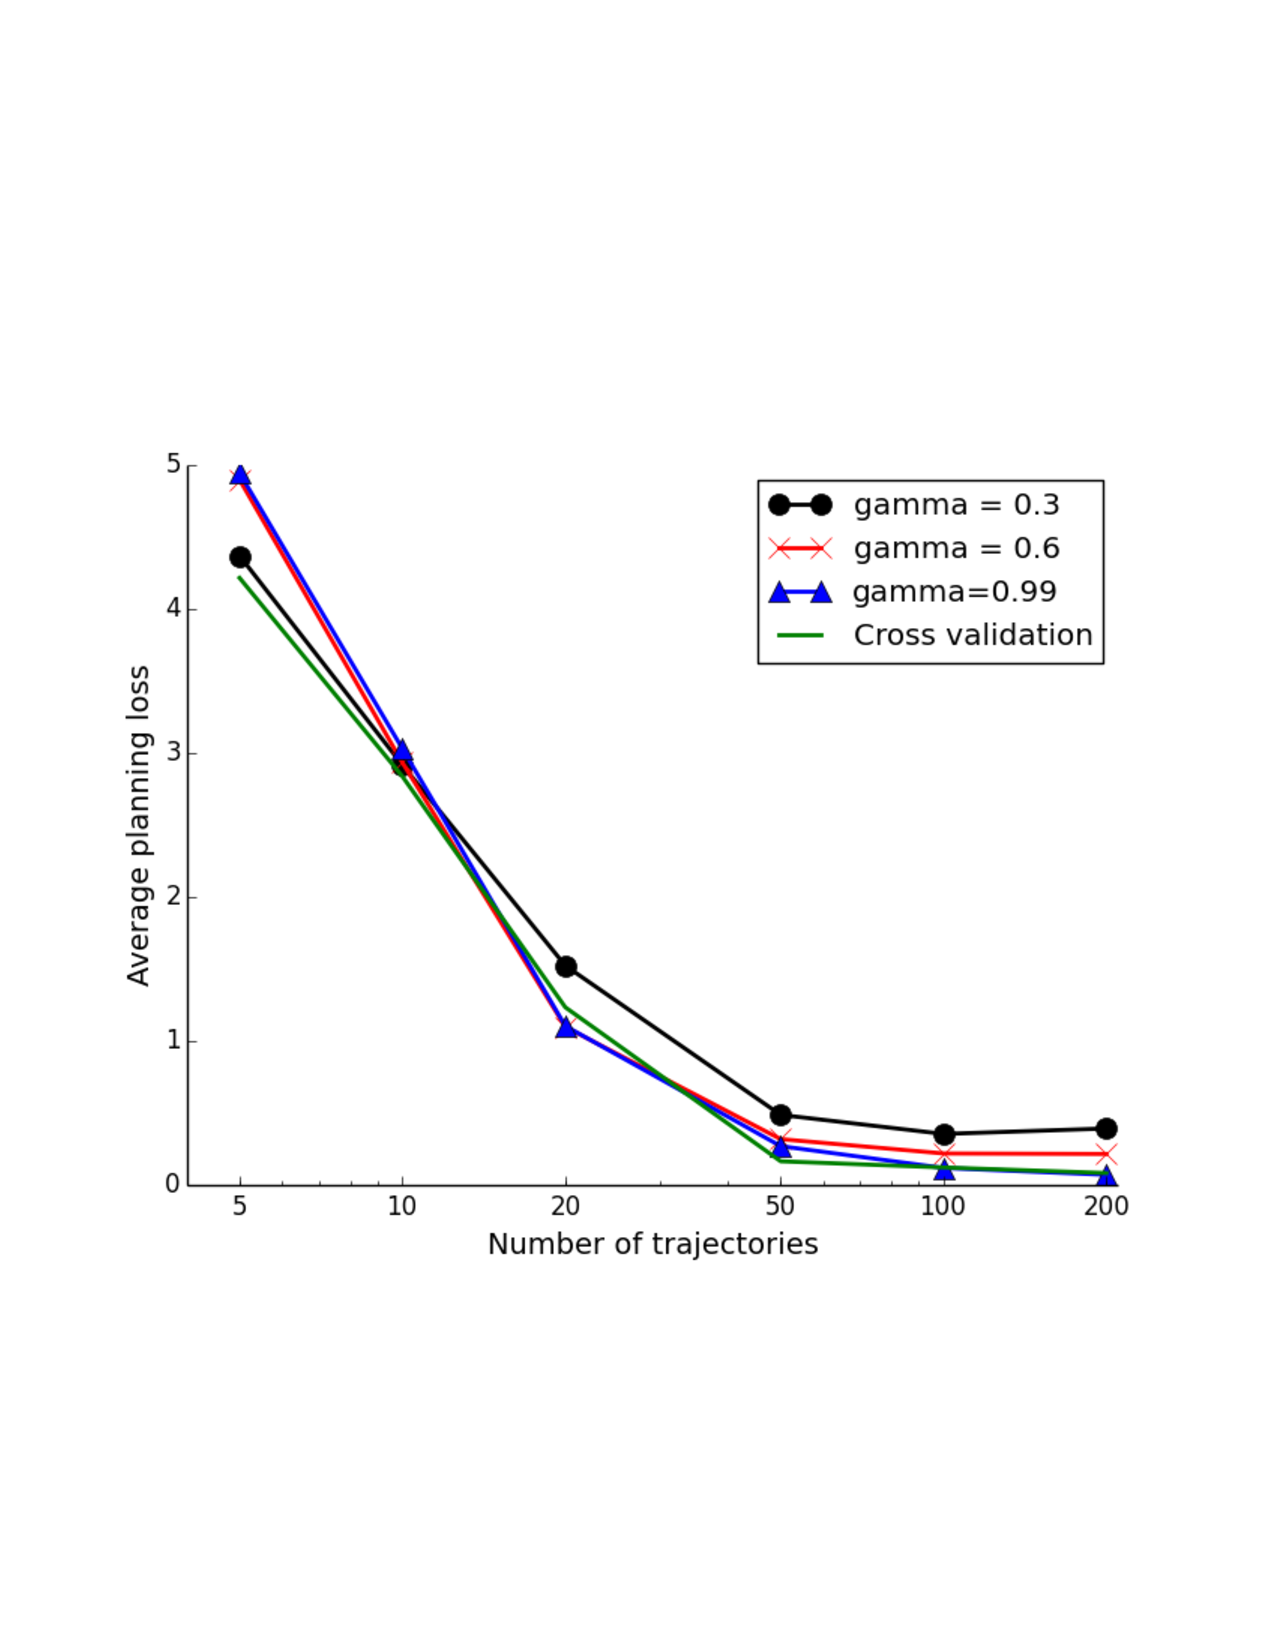
\includegraphics[page=1,width=.5\textwidth]{../results/figure_2.pdf} &
	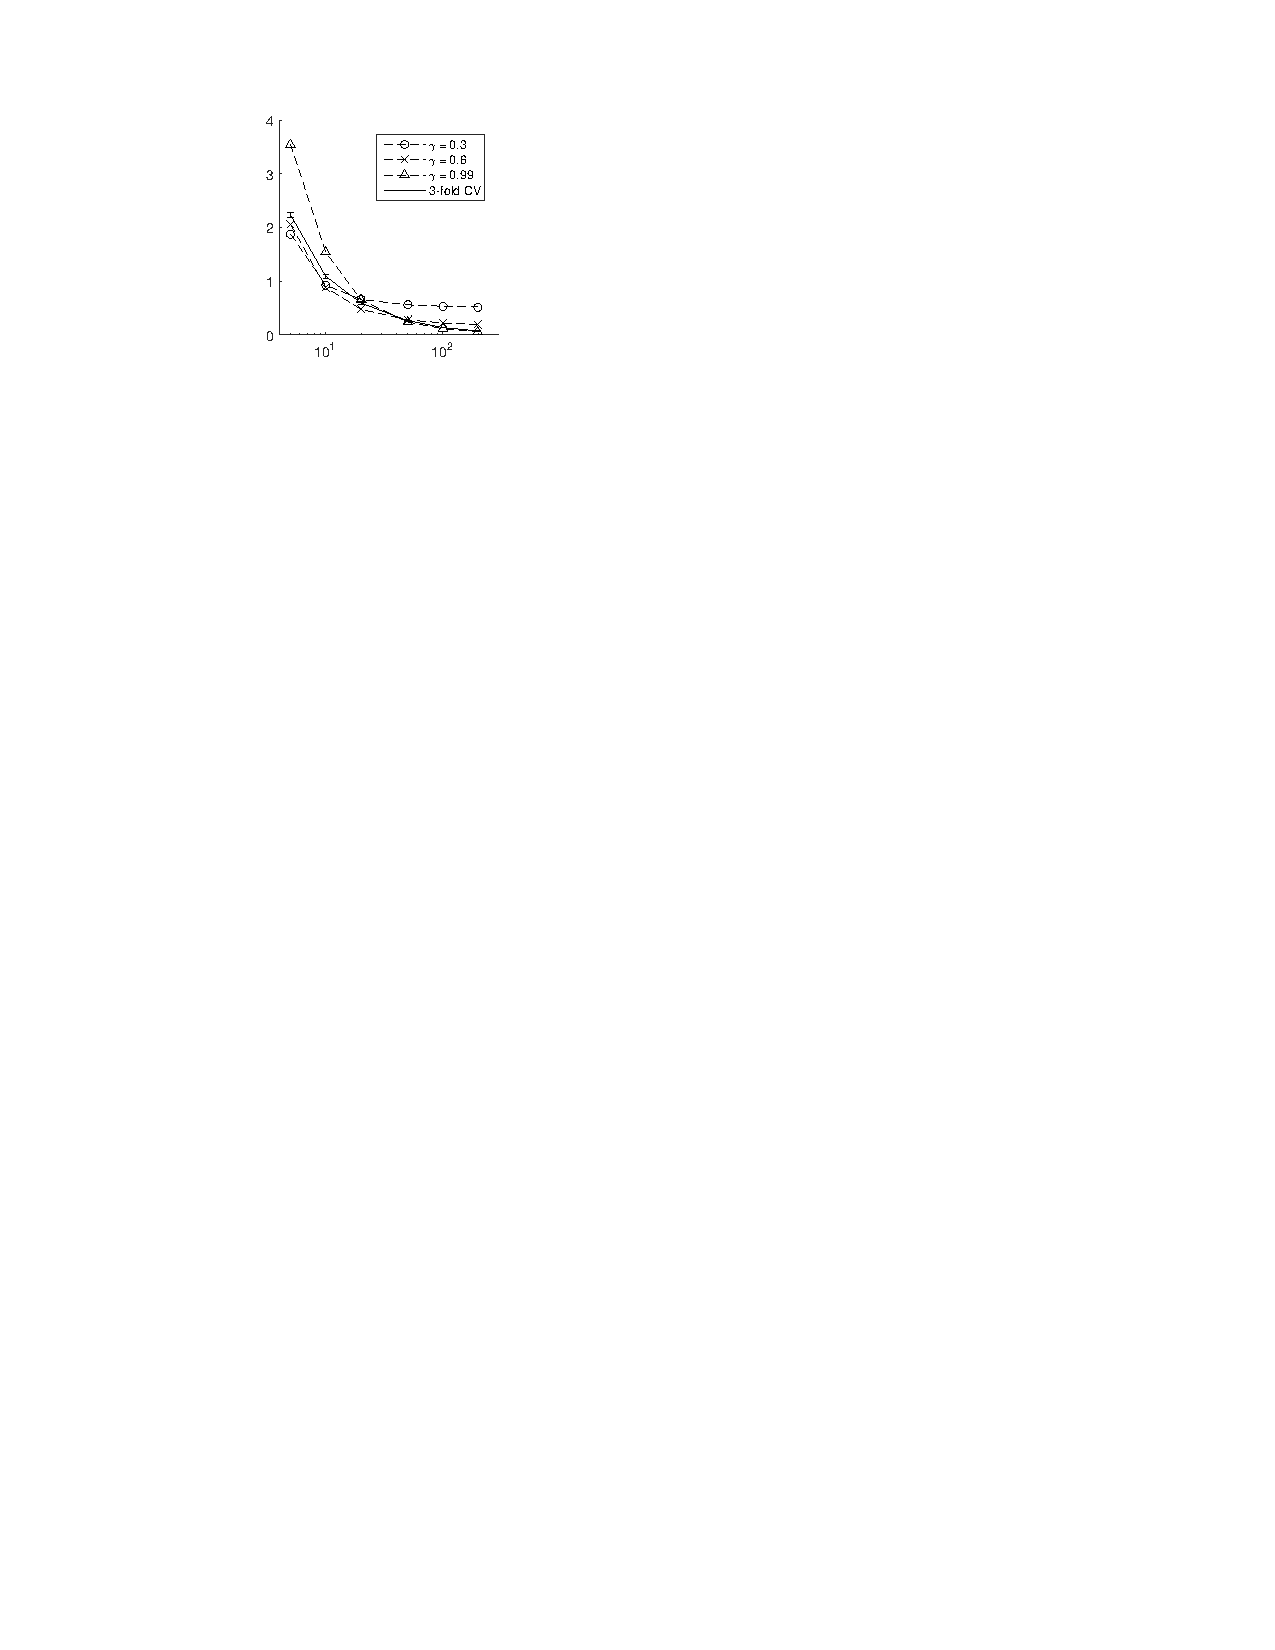
\includegraphics[page=1,width=.41\textwidth]{../results/originalCV.pdf}\\
	our results & their results \\
\end{tabular}$$


% --- SECTION: Reproducibility Discussion ---
\section{Reproducibility Discussion}

Discussion of how reproducing results was difficult, what assumptions we made, what parameters and other bits of info were left from the paper.

\subsection{Ambiguity about RockSample}
The initial state of the agent was underspecified. It was not stated whether the same initial state was used in each episode or if the state was initially randomized. In the case of the former, it was not clear what the initial state would be and in the case of the latter the distribution over states and number of rocks was indeterminate. We consulted the authors on this and were able to to determine that the same initial state with 6 rocks at fixed locations was used (this results in ~16,000 underlying states which is huge, see later Section \ref{sec: compLim} on why this is problematic). Similarly, the initial goodness of rocks was not specified -- we assumed all rocks are initially good.

There was additional ambiguity regarding the the fidelity falloff of the $Check$ actions. We assumed the distance between the agent and a rock (which determines how unreliable the sensor is) is measured using Euclidean distance. We could have also reasonably used Manhattan distance since the agent cannot move diagonally. It was also unclear what the decay rate for exponential falloff was; we used $\frac{1}{2}$.

\subsection{Ambiguity about UCT}
\begin{itemize}
\item Actual values of UCT exploration bias
\item Gamma
\item Treatment of POMDP with UCT (belief MDP?)

\subsection{General Computational Limits in RockSample}
\label{sec: compLim}
Their computer big and fast our computer small and slow.

\end{itemize}



% --- SECTION: Conclusion ---
\section{Conclusion}


% --- BIBLIOGRAPHY ---
\bibliographystyle{acm}
\bibliography{lsdm_final}

\end{document}